\documentclass{article} % For LaTeX2e
% We will use NIPS submission format
\usepackage{nips13submit_e,times}
% for hyperlinks
\usepackage{hyperref}
\usepackage{url}
% For figures
\usepackage{graphicx} 
\usepackage{subfigure} 
% math packages
\usepackage{amsmath}
\usepackage{amsfonts}
\usepackage{amsopn}
\usepackage{ifthen}
\usepackage{natbib}

\title{Robust Fisher Linear Discriminant Analysis}

\author{
Jun Lu\\
EPFL \\
\texttt{jun.lu@epfl.ch} \\
\and
Chen Liu \\
EPFL \\
\texttt{chen.liu@epfl.ch} \\
}

% The \author macro works with any number of authors. There are two commands
% used to separate the names and addresses of multiple authors: \And and \AND.
%
% Using \And between authors leaves it to \LaTeX{} to determine where to break
% the lines. Using \AND forces a linebreak at that point. So, if \LaTeX{}
% puts 3 of 4 authors names on the first line, and the last on the second
% line, try using \AND instead of \And before the third author name.

\nipsfinalcopy 

\begin{document}

\maketitle

\begin{abstract}
This is the report for the course project in CS-454 Convex Optimization and its Applications. This report will focus on Fisher Linear Discriminant Analysis(Fisher LDA). We will introduce robust Fisher LDA, compare it with and demonstrate its superiority over classic version by both theoretical analysis and experiments. We will show that robust Fisher LDA can be modeled as a convex optimization problem and can be simplified by relevant theorem.
\end{abstract}

\section{Introduction}
Fisher Linear Discrimination Analysis(Fisher LDA)[1] is a simple but effective dimension reduction technique to do binary classification. It projects a dataset into a lower-dimensional space and preserve good class-separability. However, Fisher LDA's performance is too sensitive to few outliers. The robust version of Fisher LDA in [2] solves this problems by better estimating the statistical properties of the dataset like mean and covariance. It incorporates a convex optimization problem into Fisher LDA and improves its performance for unbalanced dataset.

In next two chapters, we will introduce Fisher LDA and robust Fisher LDA respectively. Chapter 4 will focus on our tricks to solve the convex optimization problems raised by robust Fisher LDA. Chapter 5 is about dataset and experiments. Finally, we analyze the result and draw a conclusion in the last chapter.

\section{Fisher LDA}
% Linear Discriminant Analysis (LDA) is most commonly used as dimensionality reduction technique in the preprocessing step for pattern classification and machine learning applications. The goal is to project a dataset onto a lower-dimensional space with good class-separability in order avoid overfitting (“curse of dimensionality”) and also reduce computational costs.
For a linear discriminant characterized by $w \in R^n$, we seek to obtain a scalar $y$ by projecting the samples onto a line $w^Tx$. Of all the possible lines we would like to select the one that maximizes the separability of the scalars. Fisher suggested maximizing the difference between the means of the projected samples, normalized by a measure of the within-class scatter, where the within-class scatter is defined as the sum of the cluster variance or projected samples. Thus the degree of discriminant is measured by the Fisher discriminant ratio:

\begin{equation}
\begin{split}
f(w,\Sigma_x,\Sigma_y,\mu_x,\mu_y)=\frac{w^T(\mu_x - \mu_y)(\mu_x - \mu_y)^Tw}{w^T(\Sigma_x + \Sigma_y)w}=\frac{(w^T(\mu_x - \mu_y))^2}{w^T(\Sigma_x + \Sigma_y)w} = \frac{w^TS_Bw}{w^TS_Ww}=J(w)
\end{split}
\label{fisher}
\end{equation}

where $\mu_x$ and $\Sigma_x$ denote the mean and covariance of positive instances, $\mu_y$ and $\Sigma_y$ for negative instances, $S_B$ is defined as between-class covariance matrix, $S_W$ is defined as within-class covariance matrix.

Derive and equate this criteria to 0, we get $S_W^{-1}S_Bw-J(w)w=0$. By solving this generalized eigenvalue problem yields $w^*=S_W^{-1}(\mu_x - \mu_y)$ (i.e. project it to the eigenvector with largest eigenvalue). In chapter 5, we will use classic Fisher LDA to project original data into the directions of two eigenvectors with largest eigenvalues and see why we need to project it in such direction.




%Let’s assume that our goal is to reduce the dimensions of a $d$-dimensional dataset by projecting it onto a $k$-dimensional subspace (where $k<d$). So, how do we know what size we should choose for $k$($k$ = the number of dimensions of the new feature subspace), and how do we know if we have a feature space that represents our data “well”?


%We computed eigenvectors (the components) from our data set and collect them in a so-called scatter-matrices (i.e., the in-between-class scatter matrix and within-class scatter matrix).
%Each of these eigenvectors is associated with an eigenvalue, which tells us about the “length” or “magnitude” of the eigenvectors.

%If we would observe that all eigenvalues have a similar magnitude, then this may be a good indicator that our data is already projected on a “good” feature space.

%And in the other scenario, if some of the eigenvalues are much much larger than others, we might be interested in keeping only those eigenvectors with the highest eigenvalues, since they contain more information about our data distribution. Vice versa, eigenvalues that are close to 0 are less informative and we might consider dropping those for constructing the new feature subspace.




\section{Robust Fisher LDA}
In robust Fisher LDA, we take a probabilistic view to the statistical properties like $\Sigma_x$, $\Sigma_y$, $\mu_x$ and $\mu_y$ of the dataset. Instead of using `definite' values, we use a convex set $M$ as the feasible set of these parameters i.e $(\Sigma_x,\Sigma_y,\mu_x,\mu_y) \in M$. The optimization goal is to maximize the worst-case Fisher discriminant radio.
\begin{equation}
\begin{split}
max\ min_{(\Sigma_x,\Sigma_y,\mu_x,\mu_y) \in M} f(w,\Sigma_x,\Sigma_y,\mu_x,\mu_y)\\ s.t\ w \neq 0
\end{split}
\label{robust1}
\end{equation}
According to Kim's work in [2], we use $M = \{(\Sigma_x,\Sigma_y,\mu_x,\mu_y) | (\mu_x - \bar{\mu}_x)^TP_x(\mu_x - \bar{\mu}_x) \leq 1, (\mu_y - \bar{\mu}_y)^TP_y(\mu_y - \bar{\mu}_y) \leq 1, \|\Sigma_x - \bar{\Sigma}_x\|_F \leq \delta_x, \|\Sigma_y - \bar{\Sigma}_y\|_F \leq \delta_y\}$ where $\|M\|_F = (\sum_{i,j} M_{ij}^2)^{1/2}$. Parameters in this expression is obtained by resampling[3]. We first create 100 new sets which have the same size as training set and each of them are sampled uniformly from it. For each new set, we calculate its mean and covariance matrix. $\bar{\mu}_x,\bar{\mu}_y,\bar{\Sigma}_x,\bar{\Sigma}_y$ is set as the average value of corresponding mean or variance. $P_x$, $P_y$ is calculated from covariance of mean in each new set $\Sigma_{\mu_x}$, $\Sigma_{\mu_y}$ by $P_x = \Sigma_{\mu_x} / n$ and $P_y = \Sigma_{\mu_y} / n$. $\delta_x$ and $\delta_y$ is defined as the maximum deviation from the average covariance matrix in $\|-\|_F$ metric.

It is obvious that $\Sigma_x$, $\Sigma_y$ and $\mu_x$, $\mu_y$'s constraints are independent. So we can simplify equation(\ref{robust1}) by $min_{(\Sigma_x,\Sigma_y,\mu_x,\mu_y) \in M} \frac{[w^T(\mu_x - \mu_y)]^2}{w^T(\Sigma_x + \Sigma_y)w} = \frac{min_{(\mu_x,\mu_y) \in M}[w^T(\mu_x - \mu_y)]^2}{max_{(\Sigma_x,\Sigma_y) \in M}w^T(\Sigma_x + \Sigma_y)w} = \frac{min_{(\mu_x,\mu_y)\in M} [w^T (\mu_x - \mu_y)]^2}{w^T(\Sigma_x+\Sigma_y+(\delta_x+\delta_y)I)w}$. 
\textbf{Lemma 1} Let $R(w,a,B)=\frac{(w^T a)^2}{w^T B w}$ and $(a^*, B^*)$ be the optimal of following problem:
\begin{equation}
\begin{split}
min\ a^TB^{-1}a \\ s.t\ (a,B) \in V
\end{split}
\end{equation}
Let $w^*=B^{*-1}a^*$, then $(w^*,a^*,b^*)$ satisfy the minmax property
\begin{equation}
R(w^*,a^*,B^*)=a^{*T}B^{*-1}a^*=max_{w\neq 0}min_{(a,B)\in V} R(w,a,B)=min_{(a,B)\in V}max_{w\neq 0}R(w,a,b)
\end{equation}

and the saddle point property
\begin{equation}
R(w,a^*,B^*)\leq R(w^*,a^*,B^*)\leq R(w^*,a,B), \forall w \in \mathbb{R}^n\slash\{0\}, \forall (a,B) \in V
\end{equation}

The proof of lemma 1 is in Kim's paper[2]. Let $B = \bar{\Sigma}_x + \bar{\Sigma}_y + (\delta_x + \delta_y)I$ and $a = \mu_x - \mu_y$, we can solve the max-min optimization problem (2) using this lemma. The optimal value $w^*$ is
\begin{equation}
w^* = (\bar{\Sigma}_x + \bar{\Sigma}_y + (\delta_x + \delta_y)I)^{-1}(\mu_x^* - \mu_y^*)
\end{equation}
where $\mu_x^*$ and $\mu_y^*$ is the optimal value of the following optimization problem.
\begin{equation}
\begin{split}
min\ (\mu_x - \mu_y)^T(\bar{\Sigma}_x+\bar{\Sigma}_y+(\delta_x +\delta_y)I)^{-1}(\mu_x - \mu_y) \\
s.t\ (\mu_x - \bar{\mu}_x)^T P_x (\mu_x - \bar{\mu}_x) \leq 1,\ (\mu_y - \bar{\mu}_y)^T P_y (\mu_y - \bar{\mu}_y) \leq 1
\end{split}
\end{equation}
Since covariance matrix is always semi-positive definite, $\bar{\Sigma}_x + \bar{\Sigma}_y + (\delta_x + \delta_y)I$, $P_x$ and $P_y$ are all semi-positive definite. So (6) is a convex optimization problem and more specifically quadratically constrained quadratic programming (QCQP) problem. Such problem can be solved in $O(n^3)$ flops.[4]

\section{Optimization Method}
To solve the convex optimization problem(7), we can use general interior point method(IPM)[4]. There is a python library called \href{http://cvxopt.org/documentation/}{cvxopt} that we can rely on to implement IPM. However, IPM is too time and computing resource consuming to solve this problem. In this chapter, we design a parametric method which is not included in paper[2] but can estimate the optimal of problem(7) quickly and effectively.

We first write the Lagrangian of problem(7): $L(\mu_x,\mu_y,\lambda,\gamma) = (\mu_x - \mu_y)^T (\bar{\Sigma}_x + \bar{\Sigma}_y + (\delta_x + \delta_y)I)^{-1}(\mu_x - \mu_y) + \lambda ((\mu_x - \bar{\mu}_x)^T P_x (\mu_x - \bar{\mu}_x) - 1) + \gamma ((\mu_y - \bar{\mu}_y)^T P_y (\mu_y - \bar{\mu}_y) -1)$. Since problem(7) is convex, so the duality gap is zero and the optimal values should satisfy Karush–Kuhn–Tucker(KKT) conditions. We list some constraints of KKT condition below.

\begin{align}
\lambda ((\mu_x - \bar{\mu}_x) P_x (\mu_x - \bar{\mu}_x) - 1) = 0 \\
\gamma ((\mu_y - \bar{\mu}_y) P_y (\mu_y - \bar{\mu}_y) - 1) = 0 \\
\frac{\partial L}{\partial \mu_x} = (\bar{\Sigma}_x + \bar{\Sigma}_y + (\delta_x + \delta_y) I )^{-1}(\mu_x - \mu_y) + \lambda P_x (\mu_x - \bar{\mu}_x) = 0 \\
\frac{\partial L}{\partial \mu_y} = (\bar{\Sigma}_x + \bar{\Sigma}_y + (\delta_x + \delta_y) I )^{-1}(\mu_y - \mu_x) + \gamma P_y (\mu_y - \bar{\mu}_y) = 0
\end{align}

If $\lambda = 0$, according to equation(10), we have $(\bar{\Sigma}_x + \bar{\Sigma}_y + (\delta_x + \delta_y)I)^{-1}(\mu_x - \mu_y) = 0$. Multiply both sides by $(\bar{\Sigma}_x + \bar{\Sigma}_y + (\delta_x + \delta_y)I)$, we have $\mu_x - \mu_y = 0$ and this is contradict with the assumption that $\mu_x \neq \mu_y$. As a result, $\lambda$ has to be non-zero. That is to say, the corresponding constraint is tight and according to equation (8), we have the following equations.(same for $\gamma$)
\begin{align}
(\mu_x - \bar{\mu}_x)^T P_x (\mu_x - \bar{\mu}_x) = 1,\ (\mu_y - \bar{\mu}_y)^T P_y (\mu_y - \bar{\mu}_y) = 1
\end{align}

With equality constraint above, we can parameterize $\mu_x$ and $\mu_y$.
\begin{align}
\mu_x(k_x) = \bar{\mu}_x + \frac{k_x}{\sqrt{k_x^T P_x k_x}},\ \mu_y(k_y) = \bar{\mu}_y + \frac{k_y}{\sqrt{k_y^T P_y k_y}},\ k_x, k_y \in \mathbb{R}^n
\end{align}
Under such parametric setting, we can see that $\mu_x(k_x)$ and $\mu_y(k_y)$ always satisfy equation(12). Combine equation(13)'s substitution and optimization object of problem(7) and we can obtain a unconstrained optimization problem.
\begin{align}
\begin{split}
min_{k_x, k_y \in \mathbb{R}^n} H(k_x, k_y) = (\mu_x(k_x) - \mu_y(k_y))^T (\bar{\Sigma}_x + \bar{\Sigma}_y + (\delta_x + \delta_y) I) (\mu_x(k_x) - \mu_y(k_y))
\end{split}
\end{align}

$H(k_x, k_y)$ is not convex with respect to $k_x$ and $k_y$, but we can still use stochastic gradient descent(SGD)[5] to get a good estimate of the optimal value. The gradient of $H(k_x, k_y)$ is shown below. SGD process stops when the gradient's norm is lower than a threshold(usually $10^{-5}$).

\begin{align}
\frac{\partial H}{\partial k_x} = \frac{(k_x^T P_x k_x)I - P_x k_x k_x^T}{(k_x^T P_x k_x)^{3/2}} (\bar{\Sigma}_x + \bar{\Sigma}_y + (\delta_x + \delta_y) I) (\mu_x(k_x) - \mu_y(k_y)) \\
\frac{\partial H}{\partial k_y} = \frac{(k_y^T P_y k_y)I - P_y k_y k_y^T}{(k_y^T P_y k_y)^{3/2}} (\bar{\Sigma}_x + \bar{\Sigma}_y + (\delta_x + \delta_y) I) (\mu_y(k_y) - \mu_x(k_x))
\end{align}

\section{Experiment}
\subsection{Dataset Description}
To demonstrate and compare the performance of fisher LDA and robust fisher LDA, we used the sonar and ionosphere benchmark problems from the UCI repository (\href{www.ics.uci.edu/~mlearn/MLRepository.html}{LINK}). The two benchmark problems have 208 and 351 points, and the dimension of each data point is 60 and 34, respectively.

For the ionosphere dataset, there are 225 instances labeled class 1 (positive), 126 instances labeled class 2 (negative); for the sonar dataset, there are 111 entries labeled class 1 (positive), 97 entries labeled class 2 (negative). Both dataset is unbalanced, especially for ionosphere dataset.

To have a more intuitive view of both datasets, we use principle component analysis(PCA)[6] to project the whole dataset into 3-d space. We plot the spatial distribution of whole dataset, with positive and negative points marked as blue and red respectively shown in Fig \ref{fig:pcasonar} and \ref{fig:pcaionosphere}.  We can find the ionosphere dataset is more clustered than sonar. Later we will show robust Fisher LDA on the ionosphere has higher test accuracy than sonar.

\begin{figure}[h]
\center
\subfigure[sonar]{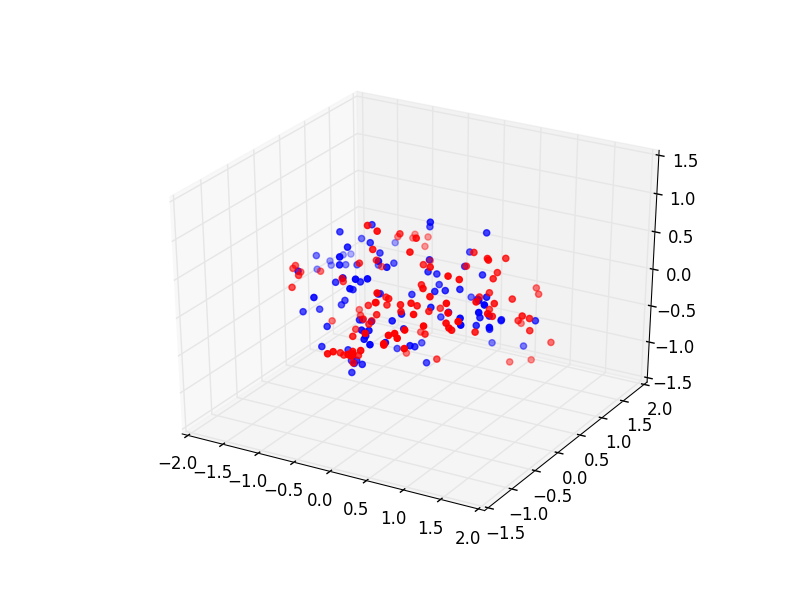
\includegraphics[width=2.6in]{figures/Sonar.png} \label{fig:pcasonar}}
\hfill
\subfigure[ionosphere]{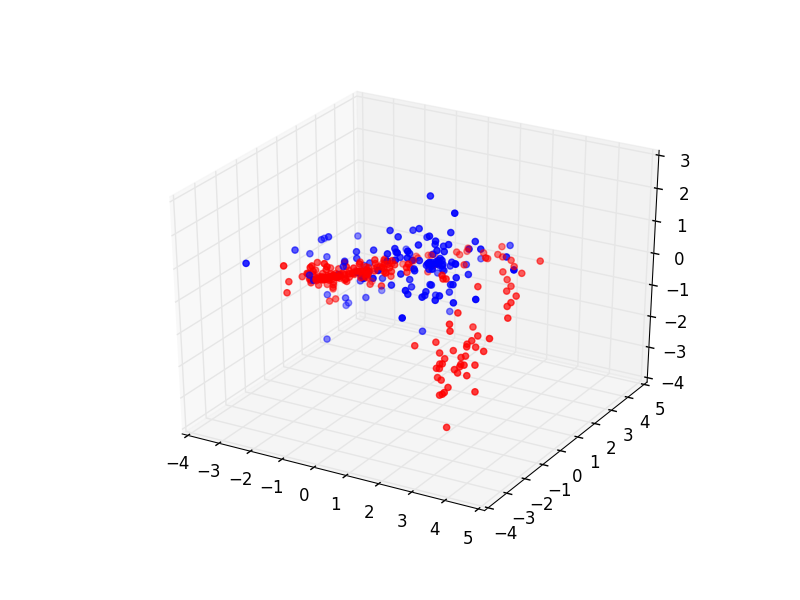
\includegraphics[width=2.6in]{figures/Ionosphere.png} \label{fig:pcaionosphere}}
\caption{PCA on two dataset into 3-d dimensions.}
\end{figure}

\subsection{Solving Unbalanced Data Set}
Concerning a linear discriminant problem, an unbalanced data set leads to biased decisions towards the majority class and therefore an increase in the generalization error. As referred in the section of Data Description, the number of samples per class in our problem is not equally distributed. To address this problem, we considered the following approaches.


$\textbf{Random Under Sampling}$ - Randomly select a subset the majority classes' data points so that the number of data points of each class is equal to the number of points of the minority class - Class 1.

$\textbf{Random Over Sampling}$ - Randomly add redundancy to the data set by duplicating data points of the minority classes so that the number of data points of each class is equal to the number of points of the majority class - Class 2.

If we compare these two methods, the \emph{Random Under Sampling} would not be useful in our problem, because the dataset is small and \emph{Random Under Sampling} will lose many information. As a result, We use \emph{Random Over Sampling} to deal with the unbalanced dataset to make the two classes equally distributed.

\subsection{Fisher LDA Numerical Results}
We sampled randomly from the dataset sonar and ionosphere separately with 60$\%$ as the training set, and 40$\%$ as the test set. After getting related two eigenvectors from the training set, we project the test set into these two directions. In Fig \ref{fig:fishersonar} and \ref{fig:fisherionosphere}, the LDA1 is the direction with largest eigenvalue, the LDA2 is the direction with the second largest eigenvalue. For the sonar dataset, if we project it to LDA1, the accuracy is 75.00$\%$; if we project it to LDA2, the accuracy is 53.57$\%$. For the ionosphere dataset, if we project it to LDA1, the accuracy is 78.01$\%$; if we project it to LDA2, the accuracy is 43.26$\%$. The vertical line in the figure is the threshold used for the direction of LDA1. From the simple test, we show the rightness of Fisher linear discriminant criterion.

\begin{figure}[h]
\center
\subfigure[sonar.]{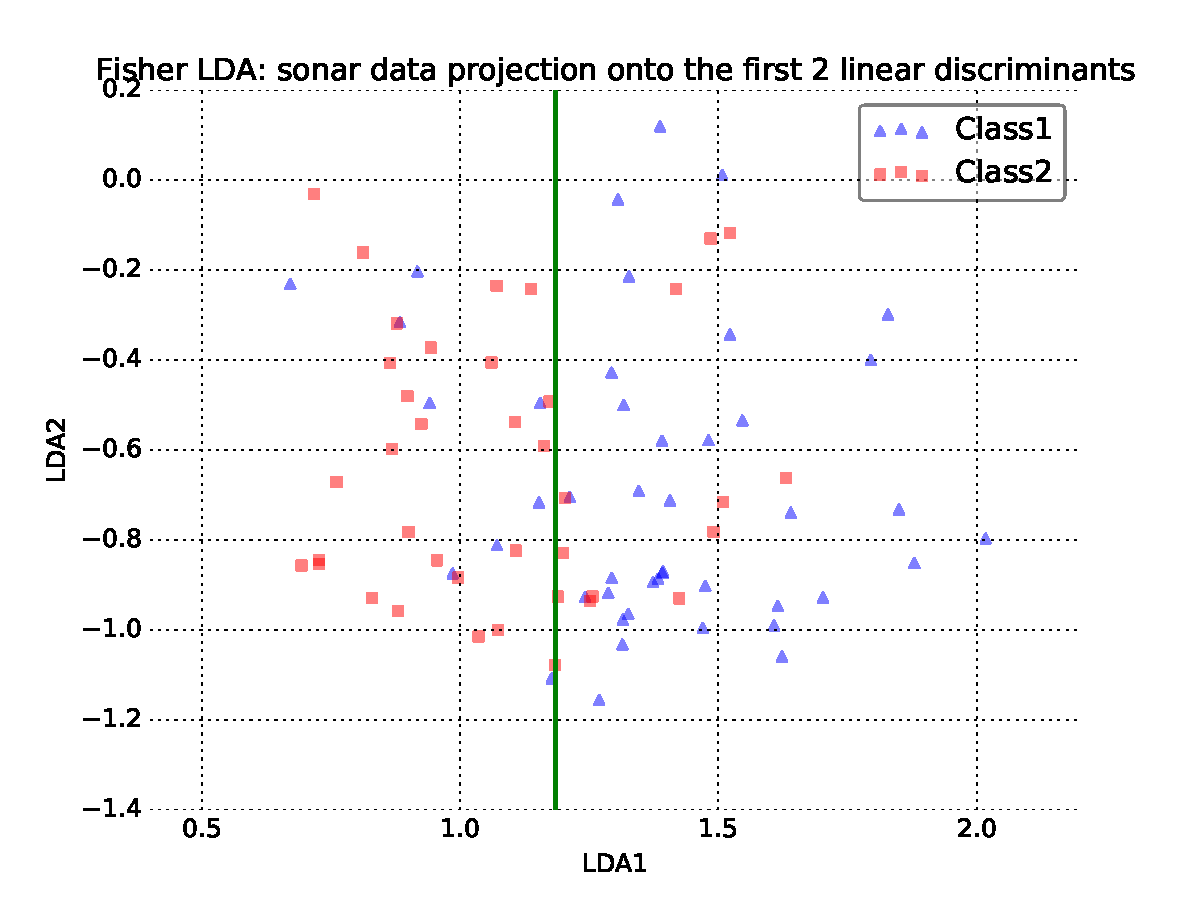
\includegraphics[width=2.6in]{figures/fishersonar.pdf} \label{fig:fishersonar}}
\hfill
\subfigure[ionosphere.]{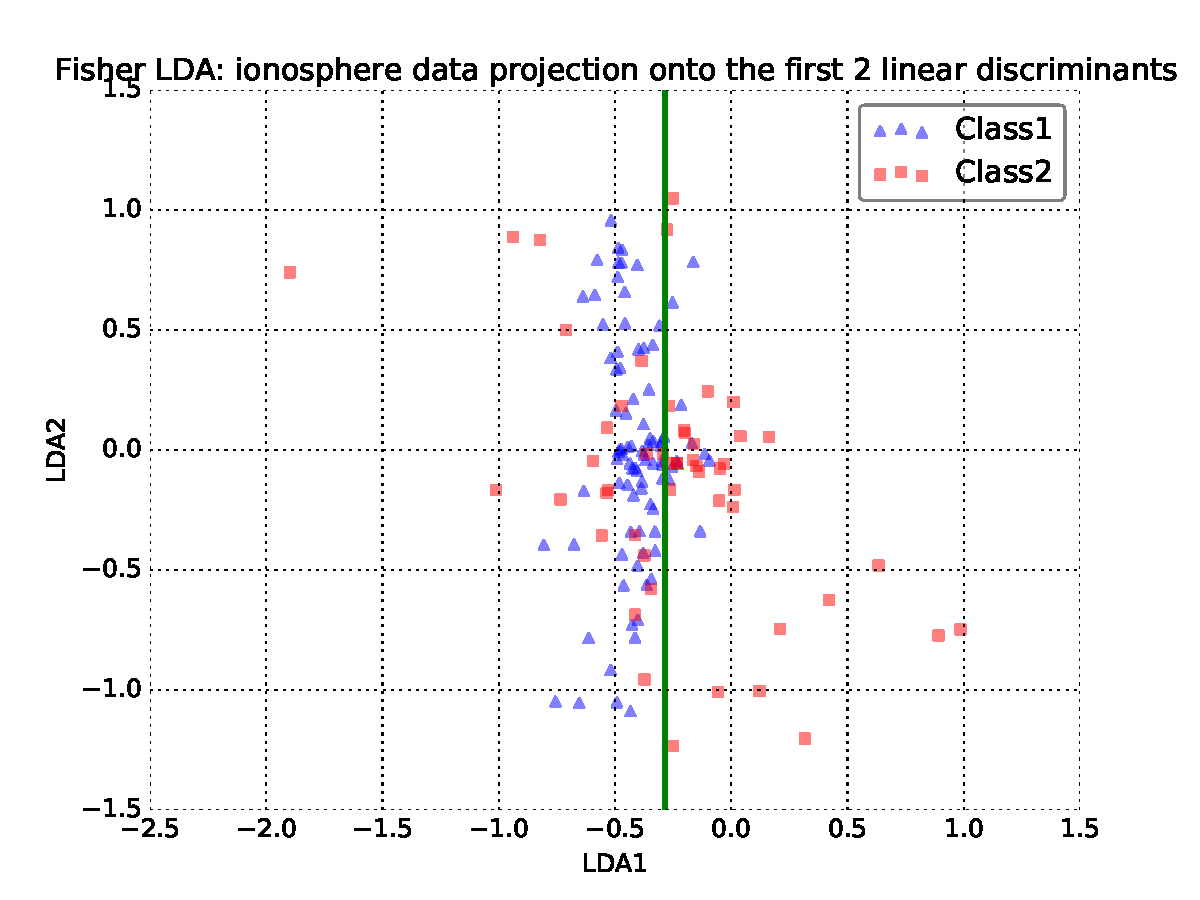
\includegraphics[width=2.6in]{figures/fisherionosphere.pdf} \label{fig:fisherionosphere}}
\caption{Project sample datas into two directions.}
\end{figure}


\subsection{Fisher LDA and Robust Fisher LDA Comparison}
To compare classic Fisher LDA and robust Fisher LDA, We test with an increasing number of training set. Fig \ref{fig:robustsonar} \ref{fig:robustionosphere} show the comparison of Test-set accuracy(TSA) between Fisher LDA and Robust Fisher LDA on the two datasets. As described in section Dataset Description, we illustrate that the Robust Fisher LDA on dataset ionosphere would have higher accuracy. Which is very clear shown in following figures.

\begin{figure}[h]
\center
\subfigure[sonar]{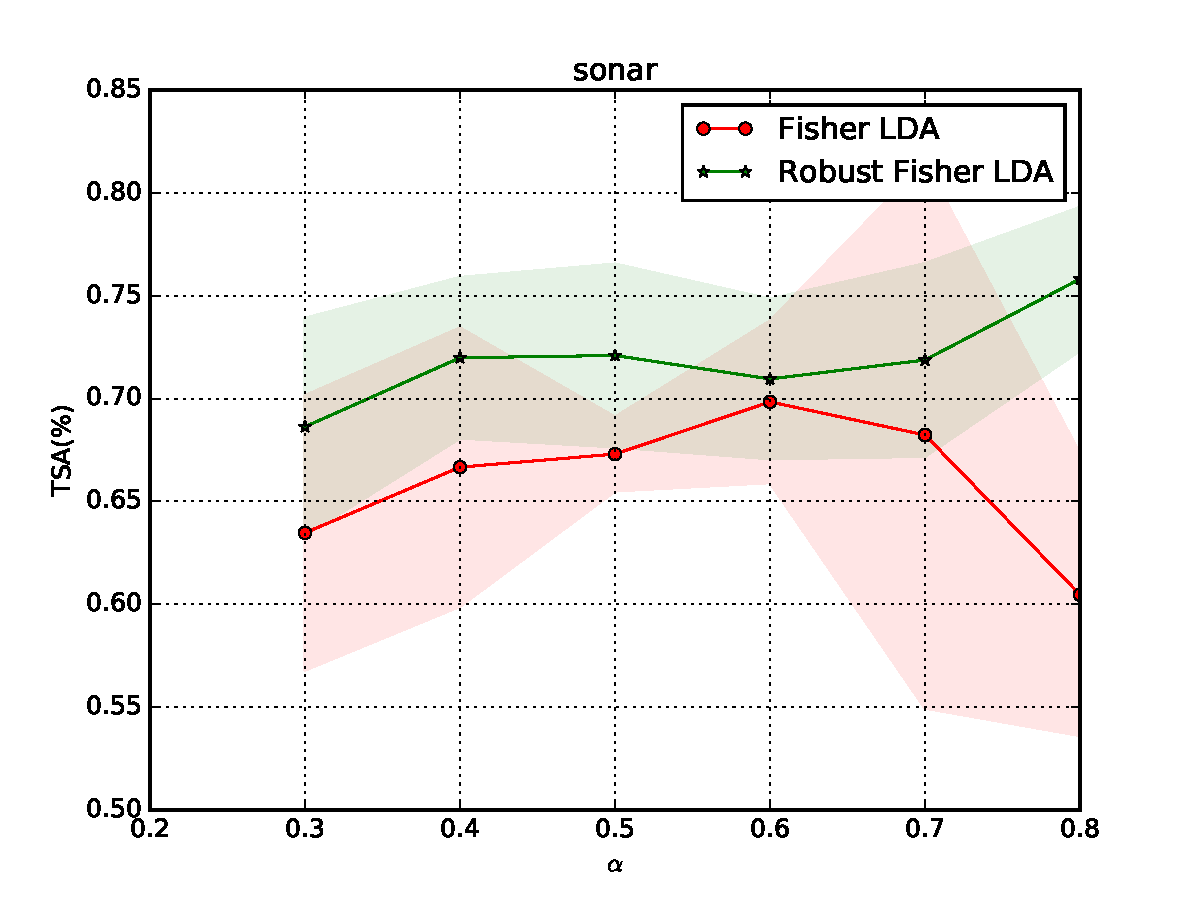
\includegraphics[width=2.6in]{figures/robustsonar.pdf} \label{fig:robustsonar}}
\hfill
\subfigure[ionosphere]{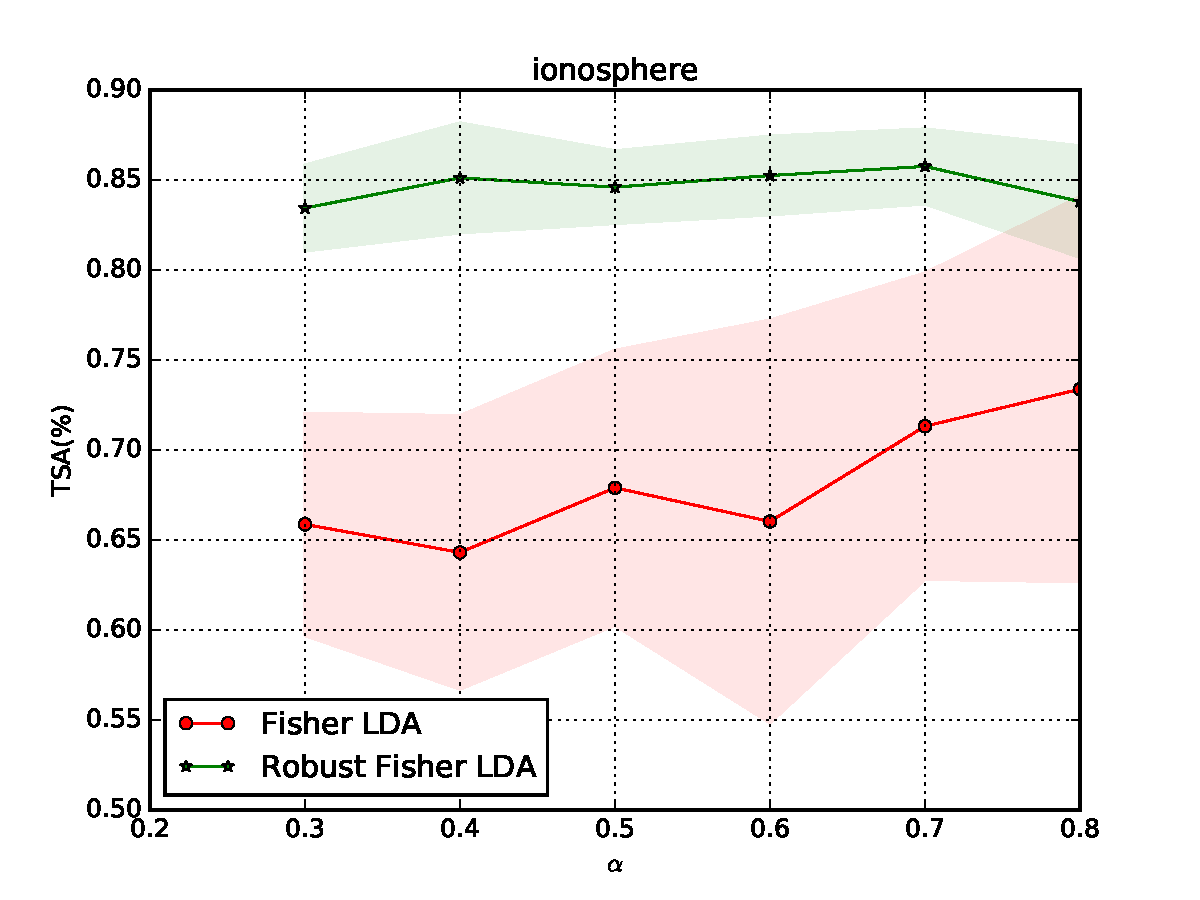
\includegraphics[width=2.6in]{figures/robustionosphere.pdf} \label{fig:robustionosphere}}
\caption{Test-set accuracy(TSA) for sonar and ionosphere for different training set size. Shadow area is the standard deviation.}
\end{figure}

\section{Conclusion}
In this project, we look into the Fisher Linear Discrimination Analysis(Fisher LDA) and use convex optimization techniques to derive and test its robust version. We have tested both models on two datasets and prove that for noisy data, robust Fisher LDA outperforms classic Fisher LDA.

\section{Reference}
[1]. Fukunaga, Keinosuke. \emph{Introduction to statistical pattern recognition.} Academic press, 2013.

[2]. MLA Kim, Seung-Jean, Alessandro Magnani, and Stephen Boyd. \emph{Robust fisher discriminant analysis.} Advances in Neural Information Processing Systems 18 (2006): 659.

[3]. B.Efron and R.Tibshirani. \emph{An Introduction to Bootstrap.} Chapman and Hall, London UK,1993.

[4]. S. Boyd and L. Vandenberghe. \emph{Convex Optimization.} Cambridge University Press, 2004.

[5]. Bottou, Léon. \emph{Large-scale machine learning with stochastic gradient descent.} Proceedings of COMPSTAT'2010. Physica-Verlag HD, 2010. 177-186.

[6]. Jolliffe, Ian. \emph{Principal component analysis.} John Wiley \& Sons, Ltd, 2002. APA

\end{document}

